% Provenance (never printed): see sources/outline_sources.md (Year 3: refraction and
% reflection seismic methods; CMP acquisition, NMO, stacking, Dix; migration in
% principle; seismic stratigraphy). Brief: sources/book5/BRIEFS.md, ch. 2. Curves from
% figdata/bachelor-3/seismic_model.py, refraction_dip.py, synthetic_seismogram.py,
% cmp_nmo.py (the Varden column, region.py); exercise and problem values in the
% Book 5 scratch calculator calc/ch02.py.
\chapter{अन्वेषण भूकंपविज्ञान}\label{ch:b3:exploration-seismology}

एक सर्वेक्षण पोत समुद्र में एक सीधी रेखा के अनुदिश धीरे-धीरे चलता है, और सतह से
कुछ मीटर नीचे एयर गनों की एक पंक्ति खींचता है, और उसके पीछे
हाइड्रोफ़ोन जड़ी कई किलोमीटर लंबी केबलें लगी होती हैं।
नियामक को वर्णित एक सर्वेक्षण में इस पंक्ति में \num{5240} घन इंच संपीडित वायु भरी थी,
हर \qty{8}{s} पर, सतह से \qty{12}{m} नीचे से दागी गई, और ऐसे पोतों के पीछे लगे
संकीर्ण-दिगंश स्ट्रीमर 8 से \qty{10}{km} तक के ऑफ़सेट पर अभिलेख करते हैं।
% ledger: noaa5:wg-survey
हर शॉट समुद्र की तली में ध्वनि का एक स्पंद भेजता है, और नीचे की हर चट्टान-सीमा
एक क्षीण प्रतिध्वनि लौटाती है। कई हफ़्तों के प्रसंस्करण के बाद एक भूवैज्ञानिक
एक अनुप्रस्थ-काट को खंगालता है, जिसमें दबी नदी-वाहिकाएँ, झुके भ्रंश-खंड और
एक पुरानी द्रोणी का \omterm{def:b3:exploration-seismology:terminations}{ऑनलैप} करता भराव ऐसे दिखाई देते हैं मानो ज़मीन चीरकर खोल दी गई हो।
पिछले अध्याय के पृथ्वी-स्तरीय भूकंपविज्ञान में भूकंपों की तरंगें प्रयुक्त हुई थीं,
जबकि अन्वेषण भूकंपविज्ञान अपनी तरंगें स्वयं उत्पन्न करता है, ऐसे स्रोतों से जिनका समय और
स्थान पूरी तरह ज्ञात होते हैं, और उन्हें हज़ारों चैनलों पर अभिलेखित किया जाता है। इस
अध्याय शॉट से अनुप्रस्थ-काट तक प्रतिध्वनियों का अनुसरण करता है: अपवर्तन सर्वेक्षण,
स्तरित स्तंभ द्वारा एक तरंगिका का परावर्तन, \omterm{def:b3:exploration-seismology:cmp}{उभयनिष्ठ मध्यबिंदु} विधि
जो दोहराई गई प्रतिध्वनियों को वेगों और एक स्वच्छ प्रतिबिंब में बदलती है, माइग्रेशन, जो
परावर्तकों को उनके सही स्थान पर लौटाता है, और अनुप्रस्थ-काट का
स्तरिकी के रूप में पठन।

\begin{recall}
दो माध्यमों की सीमा पर, जिनकी ध्वनिक प्रतिबाधाएँ $Z_1 = \rho_1v_1$ और
$Z_2 = \rho_2v_2$ हैं, अभिलंब आपतन पर एक समतल तरंग परावर्तित होती है, जिसका
आयाम गुणांक $R = (Z_2 - Z_1)/(Z_2 + Z_1)$ है (भौतिकी की पुस्तकें, वर्ष 2
की पुस्तक, सीमा पर तरंगों के विषय में)। हेड तरंग, अंतःखंड काल और
समतल परतों पर अपवर्तन-परिच्छेद की क्रॉसओवर दूरी, पुस्तक 3 (स्नातक वर्ष 1) में
स्तरित पृथ्वी वाले अध्याय में मिले थे; बोरहोल लॉग पुस्तक 2,
कक्षा 11 में। संवलन $(f*g)(t) = \int f(\tau)g(t - \tau)\,\mathrm d\tau$
और फ़ूरियर रूपांतरण गणित की पुस्तकों के विषय हैं। \omterm{def:b3:seismology-imaging:ray-parameter}{किरण प्राचल} और
रैखिक \omterm{def:b3:seismology-imaging:inverse}{प्रतिलोम समस्या} \cref{ch:b3:seismology-imaging} में आए हैं।
\end{recall}

\section{अपवर्तन सर्वेक्षण}

\begin{definition}[भूकंपीय अपवर्तन और परावर्तन सर्वेक्षण]\label{def:b3:exploration-seismology:surveys}
एक \emph{भूकंपीय अपवर्तन सर्वेक्षण}\index{भूकंपीय अपवर्तन सर्वेक्षण} ग्राहकों की एक रेखा के साथ
नियंत्रित स्रोत से आए पहले आगमनों का अभिलेख करता है, और उन हेड तरंगों का
प्रयोग करता है जो तेज़ परतों के ऊपरी भाग के साथ चलती हैं, ताकि उनकी चाल और
गहराई ज्ञात हो सके। एक \emph{भूकंपीय परावर्तन सर्वेक्षण}\index{भूकंपीय परावर्तन सर्वेक्षण}
पूरी तरंग-श्रेणी अभिलेखित करता है, मुख्यतः ऐसे ऑफ़सेट पर जो रुचि की गहराइयों से छोटे हों,
और लगभग-अभिलंब आपतन पर सीमा-तलों द्वारा परावर्तित तरंगों का
प्रयोग करता है, ताकि स्तरण का प्रतिबिंब बन सके।
\end{definition}

समतल परतों के ऊपर हेड तरंग $t = x/v_2 + t_i$ पर पहुँचती है, एक सीधी रेखा
जिसका ढलान अपवर्तक की चाल $v_2$ देता है, और जिसका अंतःखंड $t_i$
उसकी गहराई देता है। नत अपवर्तक इस रेखा को तिरछा कर देता है: नीचे-नति की ओर दागी गई
हेड तरंग देर से और देर से पहुँचती है, क्योंकि अपवर्तक गहराई में जाता है, और धीमी लगती है;
ऊपर-नति की ओर दागी गई हो तो वह तेज़ लगती है। एक ही रेखा के साथ दोनों ओर से दागकर, एक उल्टा
परिच्छेद, चाल को नति से अलग कर देता है।

\begin{theorem}[नत सीमा पर अपवर्तन]\label{thm:b3:exploration-seismology:dipping}
चाल $v_1$ की एक परत, चाल $v_2 > v_1$ वाले एक समतल अपवर्तक के ऊपर है, जो
परिच्छेद के अनुदिश कोण $\theta$ पर नत है; $i_c = \arcsin(v_1/v_2)$, और $h$
विस्फोट के नीचे अपवर्तक की लंबवत गहराई है। क्रांतिक
दूरी से परे हेड तरंग इस पर पहुँचती है
\begin{align*}
  t &= \frac{x\sin(i_c + \theta)}{v_1} + \frac{2h\cos i_c}{v_1}
  &&\text{नीचे-नति की ओर दागने पर},\\
  t &= \frac{x\sin(i_c - \theta)}{v_1} + \frac{2h\cos i_c}{v_1}
  &&\text{ऊपर-नति की ओर दागने पर}।
\end{align*}
उल्टे परिच्छेद की आभासी चालें $v_d = v_1/\sin(i_c + \theta)$ और
$v_u = v_1/\sin(i_c - \theta)$ निम्नलिखित देती हैं
\[
  i_c = \tfrac12\left[\arcsin\frac{v_1}{v_d} + \arcsin\frac{v_1}{v_u}\right],\qquad
  \theta = \tfrac12\left[\arcsin\frac{v_1}{v_d} - \arcsin\frac{v_1}{v_u}\right],
  \qquad v_2 = \frac{v_1}{\sin i_c} .
\]
\end{theorem}

\begin{proof}
फ़्रेम को इस प्रकार घुमाया जाता है कि अपवर्तक क्षैतिज हो; तब सतह
$\theta$ पर नत होती है, और नीचे-नति की ओर दागने पर ग्राही के नीचे की लंबवत गहराई, जो
ऑफ़सेट $x$ पर $h + x\sin\theta$ है, अपवर्तक पर इसका प्रक्षेप
$x\cos\theta$ है। हेड-तरंग पथ क्रांतिक कोण $i_c$ पर नीचे, अभिलंब तक जाता है,
अपवर्तक के अनुदिश $v_2$ चाल से, और $i_c$ पर ऊपर को। इसका समय है
\[
  t = \frac{h}{v_1\cos i_c} + \frac{x\cos\theta - h\tan i_c - (h + x\sin\theta)\tan i_c}{v_2}
  + \frac{h + x\sin\theta}{v_1\cos i_c}.
\]
$1/v_2 = \sin i_c/v_1$ और $1/\cos i_c - \sin i_c\tan i_c = \cos i_c$ लेने पर,
$h$ वाले पद $2h\cos i_c/v_1$ देते हैं, और $x$ वाले पद
$x(\sin i_c\cos\theta + \cos i_c\sin\theta)/v_1 = x\sin(i_c + \theta)/v_1$ देते हैं।
ऊपर-नति की ओर $\theta$ का चिह्न बदल जाता है। अंतिम सूत्र दोनों
आभासी चालों से ये राशियाँ निकालते हैं।
\end{proof}

उल्टे परिच्छेद की दोनों शाखाएँ, दोनों शॉट-बिंदुओं के बीच, एक ही समय देनी चाहिए,
चाहे किसी भी सिरे से दागा गया हो: \emph{पारस्परिक समय}, पिकिंग की
जाँच। दो स्थितियाँ इस विधि को विफल कर देती हैं। एक परत जो अपने ऊपर की परत से धीमी हो
(वेग प्रतिलोमन) कोई हेड तरंग अपवर्तित नहीं करती और अदृश्य रहती है: उसकी चट्टानें
ऊपर की परत में गिन ली जाती हैं, और नीचे की हर गहराई अधिक आंकी जाती है। एक परत
जो अपने ऊपर की परत से तेज़ हो, पर बहुत पतली हो, कभी पहला आगमन नहीं दे सकती, क्योंकि
गहरी, तेज़ परत की हेड तरंग उसे पीछे छोड़ देती है: एक छिपी परत। एक
परावर्तन सर्वेक्षण दोनों को देख सकता है।

\begin{omfigure}
\begin{tikzpicture}
\begin{axis}[omrecord, width=0.82\linewidth, height=0.46\linewidth,
  xmin=0, xmax=1200, ymin=0, ymax=660,
  xlabel={विस्तार के साथ स्थिति, पश्चिमी शॉट से (\unit{m})},
  ylabel={समय (\unit{ms})}, legend pos=north west, legend cell align=left,
  legend style={font=\scriptsize}]
\addplot[gray, thick, densely dashed] table[x=x, y=tdir] {figdata/out/bachelor-3-refraction_dip-west.dat};
\addlegendentry{प्रत्यक्ष तरंगें ($v_1$)}
\addplot[blue!70!black, thick] table[x=x, y=thead] {figdata/out/bachelor-3-refraction_dip-west.dat};
\addlegendentry{पश्चिम से हेड तरंग, ऊपर-नति शॉट}
\addplot[red!70!black, thick] table[x expr=1200-\thisrow{x}, y=thead] {figdata/out/bachelor-3-refraction_dip-east.dat};
\addlegendentry{पूर्व से हेड तरंग, नीचे-नति शॉट}
\addplot[gray, thick, densely dashed, forget plot] table[x expr=1200-\thisrow{x}, y=tdir] {figdata/out/bachelor-3-refraction_dip-east.dat};
\addplot[only marks, mark=*, mark size=1.5pt] coordinates {(1200,486.13) (0,486.13)};
\node[font=\scriptsize, anchor=south east] at (axis cs:1190,530) {पारस्परिक समय};
\end{axis}
\end{tikzpicture}

\par\smallskip{\small वार्डन अपनति के पश्चिमी अंग पर एक उलटा अपवर्तन परिच्छेद
(परिकलित; समस्या, भाग I)। अपवर्तक, अर्थात चूना-पत्थर का ऊपरी तल,
\qty{1200}{m} के विस्तार के नीचे पश्चिम से पूर्व की ओर \ang{10.8} पर ऊपर उठता है;
उसके ऊपर की चॉक और शेल को \qty{2.40}{km.s^{-1}} की एक ही परत में समेटा गया है।
पश्चिम से ऊपर-नति की ओर चलाए गए शॉट की हेड तरंग तेज़ (\qty{6.57}{km.s^{-1}}) दिखती है,
और पूर्व से नीचे-नति की ओर चलाए गए शॉट की हेड तरंग धीमी (\qty{3.52}{km.s^{-1}}) दिखती है;
दोनों को पूरे विस्तार को पार करने में \qty{486.1}{ms} लगते हैं। हेड तरंगें प्रत्यक्ष तरंगों को
केवल दूर के सिरे के पास पीछे छोड़ती हैं: इतने छोटे विस्तार के लिए अपवर्तक गहरा है।}
\label{fig:b3:exploration-seismology:refraction}
\end{omfigure}

\section{अभिलंब आपतन पर परावर्तन}

\begin{definition}[भूकंपीय तरंगिका, रिकर तरंगिका]\label{def:b3:exploration-seismology:wavelet}
एक \emph{भूकंपीय तरंगिका}\index{भूकंपीय तरंगिका} वह छोटा स्पंद है, जो कुछ दसियों
मिलीसेकंड लंबा होता है और जिसे स्रोत तथा अभिलेखन तंत्र ज़मीन में भेजते हैं;
प्रत्येक परावर्तक उसकी एक मापित प्रतिलिपि लौटाता है। \emph{रिकर
तरंगिका}\index{रिकर तरंगिका} वह शून्य-कला स्पंद है, जिसकी शिखर आवृत्ति $f$ है
\[
  w(t) = \left(1 - 2\pi^2f^2t^2\right)e^{-\pi^2f^2t^2},
\]
और वह चिह्न और मापनी को छोड़कर एक गाउसियन का द्वितीय अवकलज है: एक केंद्रीय शिखर और
दो पार्श्व लोब, जिनका माध्य शून्य है और जिसका आयाम स्पेक्ट्रम $f$ पर शिखर बनाता है।
\end{definition}

\begin{definition}[परावर्तकता श्रेणी]\label{def:b3:exploration-seismology:synthetic}
एक स्तरित स्तंभ की \emph{परावर्तकता श्रेणी}\index{परावर्तकता श्रेणी} उसके अंतरापृष्ठों के
अभिलंब-आपतन परावर्तन गुणांकों $r_k$ का अनुक्रम है, जो उनके द्विगुणित ऊर्ध्वाधर
समय $\tau_k = \sum_{i \le k} 2h_i/v_i$ पर रखे जाते हैं:
$r(t) = \sum_k r_k\,\delta(t - \tau_k)$।
\end{definition}

\begin{proposition}[संवलन मॉडल]\label{prop:b3:exploration-seismology:synthetic}
यदि केवल प्राथमिक परावर्तन रखे जाएँ (बहुपरावर्तन नहीं), अभिलंब आपतन पर, बिना संचरण-हानि,
क्षीणन या प्रसरण के, और तरंगिका $w$ गहराई के साथ नहीं बदलती, तो अभिलेखित
ट्रेस तरंगिका का
\omterm{def:b3:exploration-seismology:synthetic}{परावर्तकता श्रेणी} के साथ संवलन होता है:
\[
  s(t) = \sum_k r_k\,w(t - \tau_k) = (w*r)(t) .
\]
इस प्रकार बोरहोल लॉग के वेग और घनत्व से परिकलित ट्रेस
उस लॉग का \emph{संश्लेषित भूकंपलेख}\index{संश्लेषित भूकंपलेख} होता है।
\end{proposition}

\begin{proof}
प्रत्येक अंतरापृष्ठ आपतित तरंगिका की एक प्रतिलिपि उसके गुणांक से मापकर लौटाता है और उसके द्विगुणित समय से विलंबित करता है;
अभिलेखन रैखिक है, इसलिए प्रतिलिपियाँ जुड़ती हैं।
योग $w$ का भारित डिराक आवेगों की श्रृंखला
$r(t)$ के साथ संवलन है, क्योंकि $w*\delta(\cdot - \tau_k) = w(\cdot - \tau_k)$।
\end{proof}

\omterm{prop:b3:exploration-seismology:synthetic}{संश्लेषित भूकंपलेख} यह दिखाता है कि बोरहोल को भूकंपीय परिच्छेद से कैसे जोड़ा जाता है:
परिच्छेद पर एक परावर्तन को उस लॉग के अंतरापृष्ठ से मिलाया जाता है जो उसे उत्पन्न करता है।
इस समस्या के अभिनति-अक्ष के नीचे का वार्डन स्तंभ (इस अध्याय का भूकंपीय मॉडल,
जिसमें वेग और घनत्व प्रत्येक चट्टान के लिए
प्रकाशित परासों के भीतर चुने गए हैं)
% ledger: mavko:velocities
नीचे का चित्र दिखाता है। चॉक-शेल अंतरापृष्ठ आयाम का केवल
\qty{2.8}{\percent} परावर्तित करता है, क्योंकि चॉक और शेल का प्रतिबाधा लगभग
एक-सा होता है; चूना-पत्थर का ऊपरी तल \qty{38}{\percent} परावर्तित करता है,
चूना-पत्थर का आधार एक उलटा स्पंद लौटाता है, और आधार शिला एक
प्रबल धनात्मक स्पंद।

\begin{omfigure}
\begin{tikzpicture}
\begin{groupplot}[group style={group size=3 by 1, horizontal sep=0.45cm, y descriptions at=edge left},
  width=0.36\linewidth, height=0.6\linewidth, y dir=reverse, ymin=0.4, ymax=0.85,
  tick label style={font=\scriptsize}, label style={font=\small}, title style={font=\small}]
\nextgroupplot[title={प्रतिबाधा}, xlabel={\scriptsize $10^6$\,\unit{kg.m^{-2}.s^{-1}}},
  ylabel={द्विगुणित समय (\unit{s})}, xmin=4, xmax=14]
\addplot[black, thick] table[x=imp, y=t] {figdata/out/bachelor-3-synthetic_seismogram-log.dat};
\node[font=\tiny, anchor=west] at (axis cs:5.1,0.45) {चॉक};
\node[font=\tiny, anchor=west] at (axis cs:5.4,0.535) {शेल};
\node[font=\tiny, anchor=east] at (axis cs:11.6,0.62) {चूना-पत्थर};
\node[font=\tiny, anchor=west] at (axis cs:7.0,0.70) {बलुआ पत्थर};
\node[font=\tiny, anchor=east] at (axis cs:13.1,0.79) {शिस्ट};
\nextgroupplot[title={परावर्तकता}, xmin=-0.45, xmax=0.45, xtick={-0.4,0,0.4}]
\addplot[xcomb, red!70!black, thick, mark=*, mark size=1.2pt] table[x=r, y=t] {figdata/out/bachelor-3-synthetic_seismogram-refl.dat};
\draw[gray] (axis cs:0,0.4) -- (axis cs:0,0.85);
\nextgroupplot[title={संश्लेषित ट्रेस}, xmin=-0.45, xmax=0.45, xtick={-0.4,0,0.4}]
\addplot[blue!70!black, thick] table[x=s, y=t] {figdata/out/bachelor-3-synthetic_seismogram-trace.dat};
\draw[gray] (axis cs:0,0.4) -- (axis cs:0,0.85);
\end{groupplot}
\end{tikzpicture}

\par\smallskip{\small अभिनति-अक्ष के नीचे के वार्डन स्तंभ का \omterm{prop:b3:exploration-seismology:synthetic}{संश्लेषित भूकंपलेख}
(परिकलित)। बाएँ: प्रत्येक परत का प्रतिबाधा द्विगुणित
समय के विरुद्ध। मध्य: \omterm{def:b3:exploration-seismology:synthetic}{परावर्तकता श्रेणी}, प्रत्येक अंतरापृष्ठ पर एक शूल (शूल
प्रतिबाधा में वृद्धि के लिए दाईं ओर इंगित करते हैं)। दाएँ: \qty{30}{Hz} \omterm{def:b3:exploration-seismology:wavelet}{रिकर
तरंगिका} के साथ उनका संवलन। प्रत्येक परावर्तन तरंगिका की एक प्रतिलिपि है;
क्षीण चॉक-शेल परावर्तन, \qty{0.488}{s} पर, मुश्किल से दिखता है।}
\label{fig:b3:exploration-seismology:synthetic}
\end{omfigure}

कोई परत कितनी पतली हो सकती है और फिर भी परावर्तन उसे विभेदित कर सकें? उसके ऊपरी और निचले तल
प्रत्येक एक तरंगिका लौटाते हैं; जब वे अधिव्यापित होते हैं, तो वे व्यतिकरण करते हैं।

\begin{definition}[समस्वरण मोटाई]\label{def:b3:exploration-seismology:resolution}
किसी संस्तर की \emph{समस्वरण मोटाई}\index{समस्वरण मोटाई} वह मोटाई है, जिस पर उसके ऊपरी और निचले तल के परावर्तन,
विपरीत चिह्नों के, सबसे अधिक रचनात्मक व्यतिकरण करते हैं, ताकि संयुक्त आयाम सबसे बड़ा हो।
इससे पतले संस्तर विभेदित नहीं होते: उनके ऊपरी और निचले तल अलग-अलग
नहीं पहचाने जा सकते, और
आयाम मोटाई के अनुपात में घटता है।
\end{definition}

\begin{proposition}[चौथाई-तरंगदैर्घ्य नियम]\label{prop:b3:exploration-seismology:tuning}
प्रभावी आवर्तकाल $T$ की तरंगिका के लिए, जो $v$ वेग वाले संस्तर में है,
जिसके ऊपरी तल पर परावर्तन गुणांक $+R$ और आधार पर $-R$ हैं, संयुक्त परावर्तन
सबसे प्रबल तब होता है जब संस्तर की मोटाई $b = \lambda/4$ हो, जहाँ $\lambda = vT$;
$b \ll \lambda/4$ के लिए उसका आयाम $b$ के समानुपाती होता है।
\end{proposition}

\begin{proof}
तरंगिका को उसकी प्रमुख हार्मोनिक $\cos(2\pi t/T)$ से निरूपित किया जाता है। दोनों
परावर्तन $R\cos(2\pi t/T) - R\cos(2\pi(t - \Delta t)/T)$ हैं, जहाँ
$\Delta t = 2b/v$ है, और इनका आयाम $2R|\sin(\pi\Delta t/T)|$ है, जो $\Delta t = T/2$ के लिए
सबसे बड़ा होता है, अर्थात $b = vT/4$; छोटे $\Delta t$ के लिए यह लगभग
$2\pi R\Delta t/T = 4\pi Rb/\lambda$ होता है।
\end{proof}

एक \omterm{def:b3:exploration-seismology:wavelet}{रिकर तरंगिका} हार्मोनिक नहीं होती, और उसकी \omterm{def:b3:exploration-seismology:resolution}{समस्वरण मोटाई}, जो नीचे दिए चित्र के पच्चर मॉडल से पढ़ी जाती है,
शिखर आवृत्ति पर तरंगदैर्घ्य के चौथाई से थोड़ी कम होती है:
\qty{30}{Hz} पर \qty{3000}{m.s^{-1}} वेग वाली चट्टान में \qty{19.5}{m},
जबकि $\lambda/4 = \qty{25}{m}$ है। भूकंपीय आँकड़ों में किलोमीटरों की गहराई से
कुछ दर्जन हर्ट्ज़ से ऊपर की खासी ऊर्जा शायद ही मिलती है, क्योंकि
चट्टानें उच्च आवृत्तियों को अवशोषित कर लेती हैं; लगभग \qty{20}{m} से पतले संस्तर
एक ही परावर्तन के रूप में दिखते हैं।

\begin{omfigure}
\begin{tikzpicture}
\begin{axis}[omrecord, width=0.74\linewidth, height=0.42\linewidth,
  xmin=0, xmax=80, ymin=0, ymax=1.8,
  xlabel={संस्तर मोटाई $b$ (\unit{m})}, ylabel={शिखर आयाम / $R$}]
\addplot[blue!70!black, thick] table[x=b, y expr=2*\thisrow{amp}] {figdata/out/bachelor-3-synthetic_seismogram-wedge.dat};
\draw[red!70!black, densely dashed] (axis cs:19.5,0) -- (axis cs:19.5,1.6);
\node[font=\scriptsize, anchor=south, red!70!black] at (axis cs:19.5,1.6) {समस्वरण, \qty{19.5}{m}};
\draw[gray, densely dotted] (axis cs:25,0) -- (axis cs:25,1.6);
\node[font=\scriptsize, anchor=west, gray!40!black] at (axis cs:25.5,0.3) {$\lambda/4 = \qty{25}{m}$};
\draw[gray] (axis cs:0,1) -- (axis cs:80,1);
\node[font=\scriptsize, anchor=south east] at (axis cs:79,1) {दो अलग तरंगिकाएँ};
\end{axis}
\end{tikzpicture}

\par\smallskip{\small पच्चर मॉडल (परिकलित): एक संस्तर, जिसका वेग
\qty{3000}{m.s^{-1}} है और जिसके ऊपरी तल पर परावर्तन गुणांक $+R$ तथा
आधार पर $-R$ हैं, जिसका प्रतिचित्रण \qty{30}{Hz} की \omterm{def:b3:exploration-seismology:wavelet}{रिकर तरंगिका} से किया गया है।
संयुक्त परावर्तन का शिखर आयाम, गुणांक $R$ के एकल परावर्तन के सापेक्ष, बहुत पतले संस्तरों के लिए शून्य से रैखिक रूप से बढ़ता है,
\omterm{def:b3:exploration-seismology:resolution}{समस्वरण मोटाई} पर चरम पर पहुँचता है
और मोटे संस्तरों के लिए दो अलग तरंगिकाओं के स्तर पर स्थिर हो जाता है।}
\label{fig:b3:exploration-seismology:wedge}
\end{omfigure}

पार्श्वतः, विभेदन उस परावर्तक की चौड़ाई से तय होता है जो
ऊर्जा को कला में वापस भेजता है।

\begin{definition}[फ़्रेनेल क्षेत्र]\label{def:b3:exploration-seismology:fresnel}
किसी परावर्तक का (प्रथम) \emph{फ़्रेनेल क्षेत्र}\index{फ़्रेनेल क्षेत्र}, जिसके लिए स्रोत और ग्राही
उसके ऊपर ऊँचाई $z$ पर एक ही स्थान पर हों, परावर्तक का वह वृत्ताकार भाग है
जो अभिलंब-आपतन बिंदु के चारों ओर है, और जहाँ से द्वि-मार्गी पथ
सामान्य पथ से आधी तरंगदैर्घ्य से कम लंबा होता है: इसके परावर्तन कला में पहुँचते हैं
और मिलकर अभिलिखित परावर्तन बनाते हैं।
\end{definition}

\begin{proposition}[फ़्रेनेल क्षेत्र की त्रिज्या]\label{prop:b3:exploration-seismology:fresnel}
प्रथम \omterm{def:b3:exploration-seismology:fresnel}{फ़्रेनेल क्षेत्र} की त्रिज्या
$r_F = \sqrt{\lambda z/2 + \lambda^2/16} \approx \sqrt{\lambda z/2}$ होती है, जहाँ
$\lambda \ll z$ है।
\end{proposition}

\begin{proof}
अभिलंब-आपतन बिंदु से दूरी $r$ पर स्थित परावर्तक का एक बिंदु
स्रोत से $\sqrt{z^2 + r^2}$ दूरी पर होता है। द्वि-मार्गी अतिरिक्त पथ
$2(\sqrt{z^2 + r^2} - z)$ है; इसे $\lambda/2$ के बराबर रखने पर
$\sqrt{z^2 + r^2} = z + \lambda/4$ मिलता है, अतः $r^2 = \lambda z/2 + \lambda^2/16$।
\end{proof}

\qty{1}{km} गहराई पर, $\lambda = \qty{100}{m}$ के लिए, \omterm{def:b3:exploration-seismology:fresnel}{फ़्रेनेल क्षेत्र}
की त्रिज्या \qty{225}{m} होती है: इससे संकीर्ण संरचनाएँ धुँधली हो जाती हैं, जब तक कि
माइग्रेशन (नीचे) क्षेत्र को संकुचित न कर दे।

\begin{omfigure}
\begin{tikzpicture}[font=\small, x=1cm, y=1cm]
\fill[brown!12] (-4.5,-3.6) rectangle (4.5,-3.0);
\draw[thick] (-4.5,-3.0) -- (4.5,-3.0);
\node[anchor=north west] at (-4.4,-3.05) {परावर्तक};
\draw[thick] (-4.5,0) -- (4.5,0);
\fill (0,0) circle (2.2pt) node[above] {स्रोत और ग्राही};
\draw[->, thick] (0,0) -- (0,-2.97);
\node[anchor=west] at (0.05,-1.5) {$z$};
\draw[blue!70!black, thick] (0,0) -- (1.9,-3.0);
\draw[blue!70!black, thick] (0,0) -- (-1.9,-3.0);
\node[anchor=west, blue!70!black] at (1.0,-1.2) {$z + \lambda/4$};
\fill[red!25, opacity=0.7] (-1.9,-3.08) rectangle (1.9,-2.92);
\draw[red!70!black] (0,-3.65) -- (0,-3.95) (1.9,-3.1) -- (1.9,-3.95);
\draw[<->, red!70!black] (0,-3.85) -- (1.9,-3.85) node[midway, below] {$r_F$};
\draw[gray, densely dashed] (-57.6:3.55) arc (-57.6:-122.4:3.55);
\end{tikzpicture}

\par\smallskip{\small प्रथम \omterm{def:b3:exploration-seismology:fresnel}{फ़्रेनेल क्षेत्र} (योजनाबद्ध): परावर्तक का वह भाग जिसकी दूरी एक ही स्थान पर स्थित
स्रोत और ग्राही से सामान्य दूरी $z$ से $\lambda/4$ से कम ही अधिक हो
(बिंदुकित चाप: त्रिज्या $z + \lambda/4$ का गोला), ताकि
द्वि-मार्गी अतिरिक्त पथ आधी तरंगदैर्घ्य से कम हो,
और उसकी प्रतिध्वनियाँ कला में पहुँचें। $\lambda$ का पैमाना बढ़ाकर दिखाया गया है।}
\label{fig:b3:exploration-seismology:fresnel}
\end{omfigure}

\section{उभयनिष्ठ मध्यबिंदु अधिग्रहण और प्रसंस्करण}

एक अकेली प्रतिध्वनि शोर में इतनी क्षीण होती है कि वह दिखाई नहीं देती।
इसलिए परावर्तन सर्वेक्षण अधोभूमि के प्रत्येक बिंदु को अलग-अलग स्रोत--ग्राही युग्मों से कई बार अभिलिखित करते हैं,
और अभिलेखों को जोड़ देते हैं।

\begin{definition}[उभयनिष्ठ मध्यबिंदु, आच्छादन गुणक]\label{def:b3:exploration-seismology:cmp}
रेखा पर $x_s$ पर स्थित स्रोत और $x_r$ पर स्थित ग्राही के लिए मध्यबिंदु
$(x_s + x_r)/2$ है और दूरी (ऑफ़सेट) $x = |x_r - x_s|$ है। \emph{उभयनिष्ठ
मध्यबिंदु}\index{उभयनिष्ठ मध्यबिंदु} (CMP) समूह उन सभी
शॉटों के ट्रेसों का समुच्चय है जिनका मध्यबिंदु एक ही है; समतल परतों पर वे सभी
अधोभूमि के एक ही बिंदु से परावर्तित होते हैं। \emph{आच्छादन गुणक (भूकंपीय आच्छादन)}\index{आच्छादन गुणक (भूकंपीय आच्छादन)}
एक समूह में ट्रेसों की संख्या है। $N$ चैनलों के साथ
ग्राही अंतराल $\Delta g$ पर, और रेखा के साथ हर $\Delta s$ पर एक शॉट हो, तो
गुणक $N\Delta g/(2\Delta s)$ होता है।
\end{definition}

\begin{omfigure}
\begin{tikzpicture}[font=\small, x=1cm, y=1cm]
\draw[thick] (-5,0) -- (5,0);
\fill[brown!10] (-5,-2.6) rectangle (5,-2.2);
\draw[thick] (-5,-2.2) -- (5,-2.2);
\node[anchor=north east] at (5,-2.25) {परावर्तक};
\foreach \off/\col in {0.8/blue!70!black, 2.0/red!70!black, 3.4/green!45!black, 4.6/orange!80!black} {
  \draw[\col, thick] (-\off,0) -- (0,-2.2) -- (\off,0);
  \fill[\col] (-\off,0) circle (2.4pt);
  \fill[\col] (\off-0.12,0) -- (\off+0.12,0) -- (\off,0.2) -- cycle;
}
\fill (0,-2.2) circle (2pt);
\draw[densely dashed] (0,0.6) -- (0,-2.2);
\node[anchor=south] at (0,0.6) {उभयनिष्ठ मध्यबिंदु};
\node[anchor=north, align=center, font=\scriptsize] at (0,-2.65) {उभयनिष्ठ गहराई-बिंदु (समतल परावर्तक)};
\node[anchor=south, font=\scriptsize] at (-4.6,0.08) {शॉट};
\node[anchor=south, font=\scriptsize] at (4.6,0.25) {ग्राही};
\end{tikzpicture}

\par\smallskip{\small \omterm{def:b3:exploration-seismology:cmp}{उभयनिष्ठ मध्यबिंदु} ज्यामिति (योजनाबद्ध): भिन्न दूरियों के चार स्रोत--ग्राही
युग्म (बिंदु, त्रिभुज) एक ही मध्यबिंदु साझा करते हैं; समतल परावर्तक पर वे सभी
उसके नीचे एक ही बिंदु से परावर्तित होते हैं। उनके ट्रेस मिलकर
चार आच्छादन गुणक वाला एक समूह बनाते हैं।}
\label{fig:b3:exploration-seismology:cmp}
\end{omfigure}

\begin{theorem}[सामान्य मूवआउट]\label{thm:b3:exploration-seismology:nmo}
समतल परावर्तक के ऊपर, गति $v$ वाली एक परत में, द्वि-मार्ग ऊर्ध्वाधर समय
$t_0$ पर, दूरी $x$ पर अभिलेखित परावर्तन इस समय पर पहुँचता है:
\[
  t(x)^2 = t_0^2 + \frac{x^2}{v^2},
\]
$(x, t)$ तल में एक अतिपरवलय है। विलंब $\Delta t = t(x) - t_0$ को
\emph{सामान्य मूवआउट}\index{सामान्य मूवआउट} कहते हैं; $x \ll vt_0$ के लिए,
$\Delta t \approx x^2/(2v^2t_0)$।
\end{theorem}

\begin{proof}
परावर्तन पथ स्रोत से मध्यबिंदु के नीचे के परावर्तन बिंदु तक जाता है और
वहाँ से ऊपर ग्राही तक लौटता है: दो भुजाएँ, जिनकी लंबाई
$\sqrt{(vt_0/2)^2 + (x/2)^2}$ है। अतः $t = (2/v)\sqrt{(vt_0/2)^2 + (x/2)^2}$ और
$t^2 = t_0^2 + x^2/v^2$ है। फिर $t - t_0 = (t^2 - t_0^2)/(t + t_0) \approx
x^2/(2v^2t_0)$।
\end{proof}

कई परतों के लिए परावर्तन समय अब ठीक-ठीक अतिपरवलीय नहीं रहता, परंतु
छोटी दूरियों पर लगभग वैसा ही होता है, तथा इसकी गति परतों के
भारित माध्य होती है।

\begin{definition}[स्टैकिंग, वर्ग-माध्य-मूल और अंतराल वेग]\label{def:b3:exploration-seismology:velocities}
किसी परत का \emph{अंतराल वेग}\index{अंतराल वेग} $v_i$ उसकी
अपनी गति है; $\Delta t_i = 2h_i/v_i$ उसके आर-पार का द्वि-मार्ग समय हो, तो
परत $n$ के आधार तक का \emph{वर्ग-माध्य-मूल वेग}\index{वर्ग-माध्य-मूल वेग}
होता है:
\[
  V_{\text{वर्ग-माध्य-मूल},n} = \left(\frac{\sum_{i\le n}v_i^2\,\Delta t_i}{\sum_{i\le n}\Delta t_i}\right)^{1/2}.
\]
किसी परावर्तन का \emph{स्टैकिंग वेग}\index{स्टैकिंग वेग} उस अतिपरवलय की गति $V$ होती है,
जिसका समीकरण $t^2 = t_0^2 + x^2/V^2$ है, जो एक
\omterm{def:b3:exploration-seismology:cmp}{उभयनिष्ठ मध्यबिंदु} समूह में उसके समयों से सबसे अच्छी तरह मेल खाता है।
\end{definition}

\begin{proposition}[छोटी दूरियों पर स्टैकिंग वेग]\label{prop:b3:exploration-seismology:rms}
समतल परतों पर $t(x)^2 = t_0^2 + x^2/V_{\text{वर्ग-माध्य-मूल}}^2 + O(x^4)$ है: छोटी
दूरियों पर \omterm{def:b3:exploration-seismology:velocities}{स्टैकिंग वेग} \omterm{def:b3:exploration-seismology:velocities}{वर्ग-माध्य-मूल वेग} होता है।
\end{proposition}

\begin{proof}
\omterm{def:b3:seismology-imaging:ray-parameter}{किरण प्राचल} $p$ के लिए, $x = \sum_i 2h_i\tan\varphi_i$ और
$t = \sum_i 2h_i/(v_i\cos\varphi_i)$, जहाँ $\sin\varphi_i = pv_i$। $p$ में दूसरी
कोटि तक, $\tan\varphi_i \approx pv_i$ और $1/\cos\varphi_i \approx 1 +
p^2v_i^2/2$, अतः $x \approx p\sum v_i^2\Delta t_i = pV_{\text{वर्ग-माध्य-मूल}}^2t_0$ और
$t \approx t_0 + \tfrac12p^2V_{\text{वर्ग-माध्य-मूल}}^2t_0$। फिर
$t^2 \approx t_0^2 + p^2V_{\text{वर्ग-माध्य-मूल}}^2t_0^2 = t_0^2 + x^2/V_{\text{वर्ग-माध्य-मूल}}^2$, जबकि
छोड़े गए पद कोटि $p^4$ के हैं, यानी $x^4$ कोटि के।
\end{proof}

\begin{theorem}[डिक्स समीकरण]\label{thm:b3:exploration-seismology:dix}
यदि $V_{n-1}$ और $V_n$ परत $n$ के ऊपरी सिरे और आधार तक के \omterm{def:b3:exploration-seismology:velocities}{वर्ग-माध्य-मूल वेग} हों,
जिनके द्वि-मार्ग समय $t_{n-1}$ और $t_n$ हैं, तो परत का \omterm{def:b3:exploration-seismology:velocities}{अंतराल वेग}
\emph{डिक्स समीकरण}\index{डिक्स समीकरण} द्वारा दिया जाता है:
\[
  v_n^2 = \frac{V_n^2t_n - V_{n-1}^2t_{n-1}}{t_n - t_{n-1}} ,
\]
और इसकी मोटाई $h_n = v_n(t_n - t_{n-1})/2$ है।
\end{theorem}

\begin{proof}
परिभाषा से $V_n^2t_n = \sum_{i\le n}v_i^2\Delta t_i$ और $V_{n-1}^2t_{n-1}
= \sum_{i\le n-1}v_i^2\Delta t_i$ है। इनका अंतर $v_n^2\Delta t_n$ है, जहाँ
$\Delta t_n = t_n - t_{n-1}$ है।
\end{proof}

वेग विश्लेषण प्रत्येक समूह में उस अतिपरवलय को खोजता है जो ऊर्जा से सबसे अच्छा
मेल खाता है: प्रत्येक परीक्षण $t_0$ और $V$ के लिए ट्रेसों को वक्र के साथ जोड़ा जाता है, और
एक संगतता माप (सेम्बलेंस) का मानचित्रण किया जाता है; विश्लेषक इसके उच्चिष्ठ चुनता है,
परावर्तक-दर-परावर्तक, एक वेग फलन बनाने के लिए। फिर NMO सुधार
हर ट्रेस के हर नमूने को $t(x)$ से $t_0$ तक खिसकाता है, जिससे परावर्तन
समतल हो जाते हैं, और प्रत्येक समूह के ट्रेस जोड़ दिए जाते हैं।

\begin{definition}[स्टैकिंग (भूकंपीय)]\label{def:b3:exploration-seismology:stack}
\emph{स्टैकिंग (भूकंपीय)}\index{स्टैकिंग (भूकंपीय)} \omterm{thm:b3:exploration-seismology:nmo}{सामान्य मूवआउट} सुधार के बाद
किसी \omterm{def:b3:exploration-seismology:cmp}{उभयनिष्ठ मध्यबिंदु} समूह के ट्रेसों का वह योग है जो एक ही ट्रेस बनाता है
जिसे मध्यबिंदु पर रखा जाता है। रेखा के साथ-साथ रखे गए स्टैक्ड ट्रेस
मिलकर स्टैक्ड खंड बनाते हैं, जो द्वि-मार्ग समय में परावर्तकों का चित्र है।
\end{definition}

\begin{proposition}[स्टैक का लाभ]\label{prop:b3:exploration-seismology:sqrtN}
यदि किसी समूह के $N$ ट्रेसों में एक ही परावर्तन संकेत और स्वतंत्र
शोर हो, जिसका समान मानक विचलन $\sigma$ है, तो उनका माध्य वही संकेत
और $\sigma/\sqrt N$ मानक विचलन का शोर ले जाता है: स्टैकिंग से
सिग्नल-से-शोर अनुपात $\sqrt N$ गुना बढ़ जाता है।
\end{proposition}

\begin{proof}
$N$ स्वतंत्र चरों के योग का प्रसरण उनके प्रसरणों का योग होता है
$N\sigma^2$ है; $N^2$ से भाग देने पर माध्य का प्रसरण $\sigma^2/N$ प्राप्त होता है
(माध्य का मानक विचलन, जो गणित की
पुस्तकों में आ चुका है)।
\end{proof}

\begin{omfigure}
\begin{tikzpicture}
\begin{groupplot}[group style={group size=2 by 1, horizontal sep=0.5cm, y descriptions at=edge left},
  width=0.52\linewidth, height=0.56\linewidth, y dir=reverse, ymin=0.4, ymax=0.92,
  xmin=-150, xmax=2150, tick label style={font=\scriptsize}, title style={font=\small},
  xlabel={\scriptsize ऑफ़सेट (\unit{m})}]
\nextgroupplot[title={(क) CMP समूह}, ylabel={द्वि-मार्ग समय (\unit{s})}]
\addplot[black, very thin, unbounded coords=jump] table[x=x, y=t] {figdata/out/bachelor-3-cmp_nmo-gather-raw.dat};
\nextgroupplot[title={(ख) NMO सुधार के बाद}]
\addplot[black, very thin, unbounded coords=jump] table[x=x, y=t] {figdata/out/bachelor-3-cmp_nmo-gather-nmo.dat};
\end{groupplot}
\end{tikzpicture}

\par\smallskip{\small वार्डन रेखा की अभिनति-अक्ष के नीचे का एक संश्लिष्ट CMP समूह
(सपाट-परतदार स्तंभ से होकर सटीक किरण-अनुरेखण द्वारा परिकलित; 30
Hz \omterm{def:b3:exploration-seismology:wavelet}{रिकर तरंगिका}; कोई शोर नहीं)। (क) चार परावर्तन (शेल का शीर्ष, चूना-पत्थर का शीर्ष
और आधार, आधारशैल का शीर्ष) ऑफ़सेट के साथ नीचे की ओर
लगभग अतिपरवलयों के अनुदिश झुकते हैं। (ख) NMO सुधार के बाद, जिसमें \omterm{def:b3:exploration-seismology:velocities}{स्टैकिंग वेग}
\qty{600}{m} तक के ऑफ़सेट पर निर्धारित किए गए थे, परावर्तन लगभग
\qty{1}{km} तक सपाट रहते हैं; उससे आगे सही काल अतिपरवलय से विचलित हो जाते हैं और
सुधार उन्हें मुड़ा हुआ छोड़ देता है, और तरंगिकाएँ खिंच जाती हैं; संसाधन में,
उथले परावर्तनों के खिंचे हुए दूर के ट्रेसों को
स्टैक से पहले म्यूट कर दिया जाता है।}
\label{fig:b3:exploration-seismology:gather}
\end{omfigure}

\begin{omfigure}
\begin{tikzpicture}
\begin{axis}[omrecord, width=0.72\linewidth, height=0.46\linewidth,
  xmin=0.4, xmax=0.78, ymin=2000, ymax=5000,
  xlabel={द्वि-मार्ग समय $t_0$ (\unit{s})}, ylabel={वेग (\unit{m.s^{-1}})},
  legend cell align=left, legend columns=2,
  legend style={font=\scriptsize, at={(0.5,-0.24)}, anchor=north}]
\addplot[gray, thick, const plot mark right] table[x=t0, y=vint] {figdata/out/bachelor-3-cmp_nmo-vel.dat};
\addlegendentry{मॉडल का अंतराल वेग}
\addplot[gray, thick, forget plot] coordinates {(0.4,2500) (0.487847,2500)};
\addplot[blue!70!black, thick, mark=*, mark size=1.5pt] table[x=t0, y=vrms] {figdata/out/bachelor-3-cmp_nmo-vel.dat};
\addlegendentry{वर्ग-माध्य-मूल वेग}
\addplot[red!70!black, only marks, mark=square*, mark size=1.6pt] table[x=t0, y=vstack] {figdata/out/bachelor-3-cmp_nmo-vel.dat};
\addlegendentry{स्टैकिंग वेग (ऑफ़सेट \qty{600}{m} तक)}
\addplot[green!45!black, only marks, mark=triangle*, mark size=2pt] table[x=t0, y=vdix] {figdata/out/bachelor-3-cmp_nmo-vel.dat};
\addlegendentry{डिक्स अंतराल वेग}
\end{axis}
\end{tikzpicture}

\par\smallskip{\small अभिनति-अक्ष के नीचे के वेग (परिकलित)। \omterm{def:b3:exploration-seismology:velocities}{वर्ग-माध्य-मूल वेग},
एक भारित माध्य है और धीरे-धीरे बदलता है; समूह के \omterm{def:b3:exploration-seismology:velocities}{स्टैकिंग वेग}
उसके निकट पड़ते हैं। इन पर लगाने पर \omterm{thm:b3:exploration-seismology:dix}{डिक्स समीकरण} प्रत्येक संस्तर का \omterm{def:b3:exploration-seismology:velocities}{अंतराल वेग}
(सीढ़ी-रेखा, जो प्रत्येक संस्तर के आधार पर खींची गई है) कुछ प्रतिशत
के भीतर पुनः प्राप्त करता है; पतले और तेज़ चूना-पत्थर में त्रुटि बढ़ती है।}
\label{fig:b3:exploration-seismology:velocities}
\end{omfigure}

\begin{omfigure}
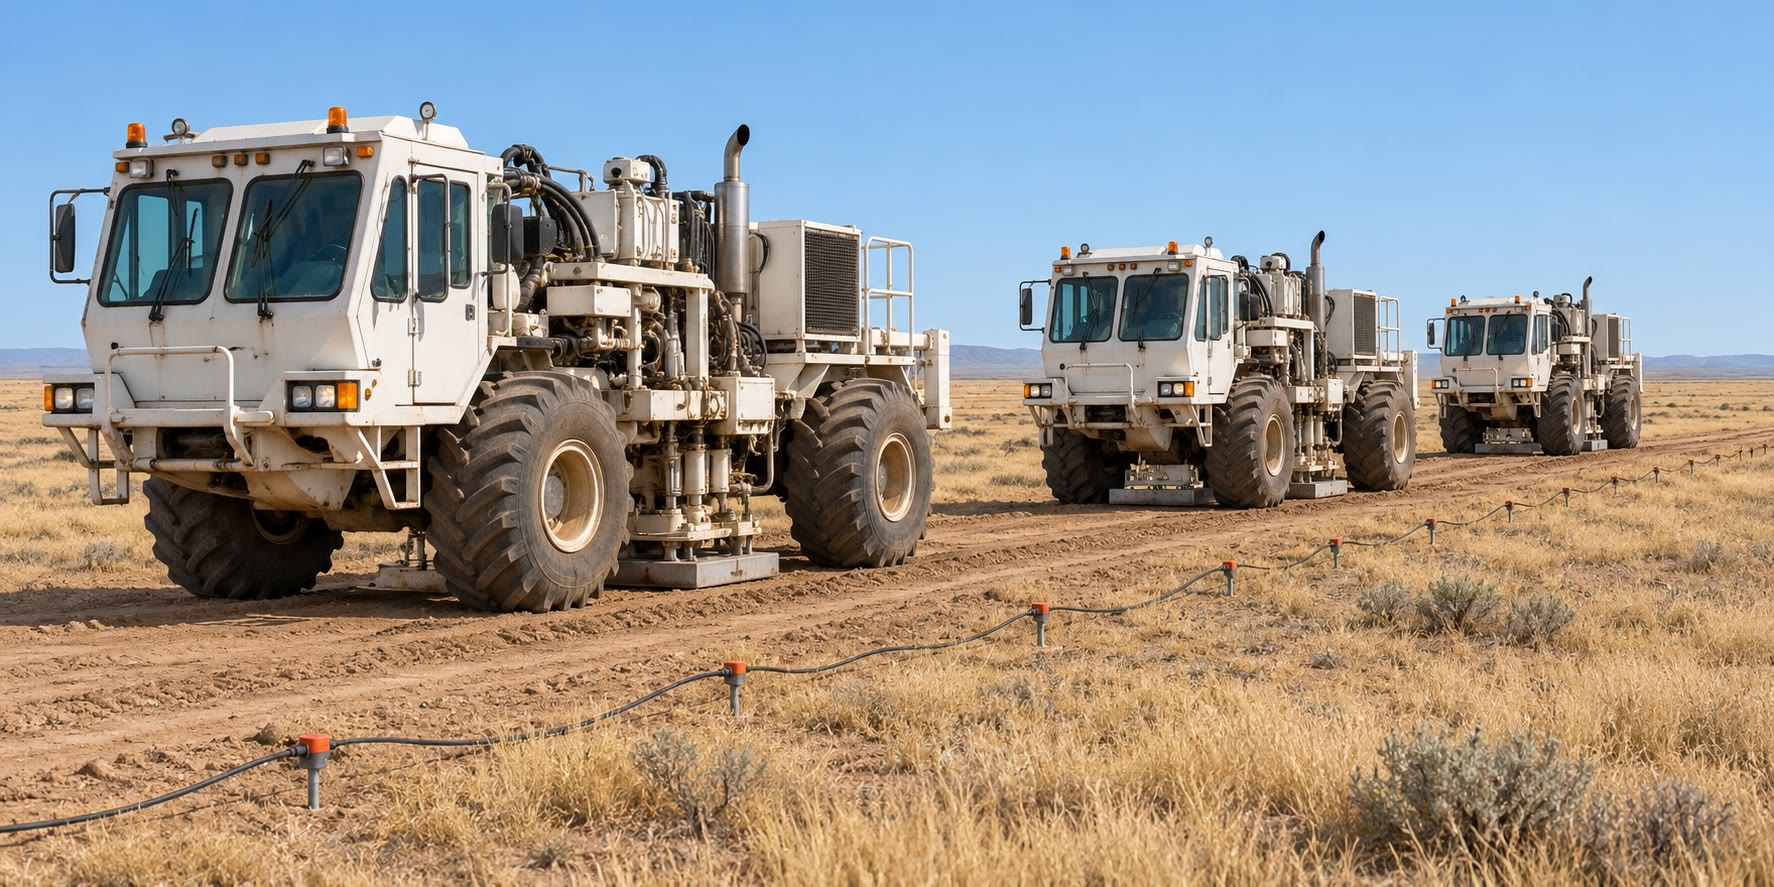
\includegraphics[width=0.62\linewidth]{images/book5/ai/b3-vibroseis.jpg}

\par\smallskip{\small भूमि सर्वेक्षण रेखा पर कंपक ट्रक: विस्फोट के बजाय
प्रत्येक ट्रक ज़मीन पर एक भारी प्लेट दबाता है और उसे आवृत्तियों के एक
स्वीप से कई सेकंड तक हिलाता है; लंबे अभिलेखों को
स्वीप के साथ सहसंबंधित करके छोटे स्पंदों में संपीड़ित किया जाता है (AI से बनाया गया चित्रण)।}
\label{fig:b3:exploration-seismology:vibroseis}
\end{omfigure}

\section{माइग्रेशन}

स्टैक्ड खंड हर परावर्तन को उस मध्यबिंदु के नीचे दिखाता है जहाँ उसे
अभिलिखित किया गया था, उस समय पर जो उसके लौटने में लगा। सपाट परावर्तक के लिए
वह वहीं है। नत परावर्तक के लिए ऐसा नहीं है: किसी सतह बिंदु पर अभिलिखित प्रतिध्वनि
परावर्तक के उस बिंदु से आती है जो उसके सबसे निकट है और जो ऊपर-नति की ओर है,
न कि ठीक नीचे। भ्रंश-कटाव जैसे बिंदु, जो सभी दिशाओं में ऊर्जा
बिखेरते हैं, अतिपरवलय के रूप में दिखाई देते हैं।

\begin{definition}[भूकंपीय माइग्रेशन]\label{def:b3:exploration-seismology:migration}
\emph{भूकंपीय माइग्रेशन}\index{भूकंपीय माइग्रेशन} वह संसाधन चरण है जो भूकंपीय खंड के
परावर्तनों को उन परावर्तकों की स्थितियों पर ले जाता है जिन्होंने उन्हें
उत्पन्न किया था: यह नत परावर्तकों की वास्तविक नतियाँ और स्थितियाँ
पुनःस्थापित करता है, और बिंदु-प्रकीर्णकों के विवर्तन अतिपरवलयों को
उनके शीर्षों पर संकुचित करता है। समय में वेग मॉडल से किए जाने पर यह समय-माइग्रेटेड
खंड देता है; गहराई में मॉडल से, गहराई-प्रतिबिंब।
\end{definition}

\begin{theorem}[शून्य-ऑफ़सेट खंड पर नति]\label{thm:b3:exploration-seismology:dip}
वेग $v$ वाले माध्यम में, खंड के समतल में नति $\theta$ वाला एक समतल परावर्तक
शून्य-ऑफ़सेट खंड पर प्रकट होता है, जिसमें गहराई $vt/2$ के रूप में आरेखित
प्रत्येक अभिलेखन बिंदु के ठीक नीचे, आभासी नति $\theta_a$ की एक रेखा के रूप में
जिसके लिए
\[
  \tan\theta_a = \sin\theta .
\]
बिंदु $x$ पर अभिलिखित परावर्तन उस परावर्तक बिंदु से आता है जो
$(vt/2)\sin\theta$ दूरी पर, $x$ के ठीक नीचे के बिंदु से ऊपर-नति की ओर स्थित है।
\end{theorem}

\begin{proof}
शून्य-ऑफ़सेट किरण परावर्तक के लंबवत होती है, इसलिए $x$ पर अभिलिखित समय
$t = 2d(x)/v$ है, जहाँ $d(x)$ $x$ से समतल तक की दूरी है। यह दूरी
$\sin\theta$ से बढ़ती है, नति-दिशा में $x$ की प्रत्येक इकाई के लिए, अतः आरेखित
गहराई $vt/2 = d(x)$ की प्रवणता $\sin\theta$ है। $x$ से लंब का
समतल पर पड़ने वाला पाद $d\sin\theta$ क्षैतिज दूरी पर, $x$ से
ऊपर-नति की ओर स्थित है।
\end{proof}

चूँकि $\tan\theta_a = \sin\theta < \tan\theta$ है, बिना माइग्रेशन का खंड सदैव
वास्तविक नतियों से मंद नतियाँ दिखाता है, और वह
\ang{45} से अधिक नति बिल्कुल नहीं दिखा सकता। गहराई $z$ पर, बिंदु $x_0$ के नीचे स्थित एक बिंदु प्रकीर्णक
$x$ पर शून्य-ऑफ़सेट समय $t(x) = (2/v)\sqrt{z^2 + (x - x_0)^2}$ लौटाता है: एक अतिपरवलय
जिसका शीर्ष उस बिंदु के ऊपर है, यही विवर्तन है। सरलतम रूप में माइग्रेशन,
जिसे विवर्तन स्टैक कहते हैं, प्रत्येक खंड को हर संभावित प्रकीर्णक के विवर्तन अतिपरवलय के
अनुदिश जोड़ता है और योग को शीर्ष पर रख देता है: परावर्तक, जो प्रकीर्णकों की
निरंतर रेखाएँ हैं, अपने वास्तविक स्थानों पर उभरते हैं, और
विवर्तन संकुचित हो जाते हैं।

\begin{omfigure}
\begin{tikzpicture}[font=\small, x=1cm, y=1cm]
\draw[thick] (-0.5,0) -- (8.5,0) node[right] {सतह};
% true reflector, dip 35 deg, rising to the left
\draw[very thick, brown!70!black] (1.0,-1.2) -- (6.0,-4.70);
\node[brown!50!black, anchor=east] at (0.95,-1.2) {सही परावर्तक};
% zero-offset normal rays from x = 2, 4, 6
\foreach \x in {2.5, 4.5, 6.5} {
  % distance from (x,0) to the line through (1,-1.2) dir (cos35,-sin35): normal n=(sin35,cos35)
  \pgfmathsetmacro{\dd}{abs(0.5736*(\x-1.0) + 0.8192*(0+1.2))}
  \draw[blue!60!black, ->] (\x,0) -- ++({-0.5736*\dd},{-0.8192*\dd});
  \fill[blue!70!black] (\x,{-\dd}) circle (1.8pt);
}
% apparent reflector through the plotted points
\pgfmathsetmacro{\da}{abs(0.5736*1.5 + 0.8192*1.2)}
\pgfmathsetmacro{\db}{abs(0.5736*5.5 + 0.8192*1.2)}
\draw[blue!70!black, thick, densely dashed] (2.5,{-\da}) -- (6.5,{-\db});
\node[blue!60!black, anchor=west] at (6.6,{-\db}) {अनपरिवर्तित};
\node[anchor=south, font=\scriptsize] at (4.5,0.05) {अभिलेखन बिंदु};
\draw[->, red!70!black, thick] (6.4,{-\db+0.05}) to[bend right=25] ({6.5-0.5736*\db+0.05},{-0.8192*\db-0.12});
\end{tikzpicture}

\par\smallskip{\small नत परावर्तक का माइग्रेशन (योजनाबद्ध, सही नति
\ang{35})। शून्य-ऑफ़सेट किरण प्रत्येक अभिलेखन बिंदु पर परावर्तक के लंबवत होती है,
इसलिए उसकी प्रतिध्वनि ऊपर-नति की ओर से आती है; बिंदु के नीचे ऊर्ध्वाधर रूप से अंकित,
गहराई $vt/2$ पर परावर्तन अधिक मंद दिखता है (बिंदीदार: $\tan\theta_a =
\sin\theta$, यहाँ \ang{29.8}), और नीचे-नति की ओर विस्थापित होता है। माइग्रेशन (लाल तीर) उसे वापस ले जाता है।}
\label{fig:b3:exploration-seismology:migration}
\end{omfigure}

\section{भूकंपीय स्तरिकी}

माइग्रेशन के बाद का खंड संस्तरण का चित्र है, और उसे स्तरिकी के रूप में पढ़ा जा सकता है:
परावर्तन संस्तरण-सतहों का अनुसरण करते हैं, जो समय-रेखाएँ हैं,
इसलिए उनकी ज्यामिति बताती है कि बेसिन कैसे भरा।

\begin{definition}[भूकंपीय स्तरिकी, भूकंपीय संलक्षणी]\label{def:b3:exploration-seismology:seismic-stratigraphy}
\emph{भूकंपीय स्तरिकी}\index{भूकंपीय स्तरिकी} किसी बेसिन की स्तरिकी और निक्षेपण-इतिहास की
व्याख्या है, जो उसके भूकंपीय परावर्तनों की ज्यामिति से की जाती है। \emph{भूकंपीय संलक्षणी}\index{भूकंपीय संलक्षणी}
परावर्तनों की एक त्रि-आयामी इकाई है जिसका स्वरूप (सततता, आयाम,
आवृत्ति, आंतरिक ज्यामिति: समांतर, अपसारी, सिग्मॉइड, अव्यवस्थित, टीलेदार)
अपने पड़ोसियों से भिन्न होता है और
उसकी व्याख्या निक्षेपण-परिवेश के रूप में
की जाती है।
\end{definition}

\begin{definition}[परावर्तक-समापन]\label{def:b3:exploration-seismology:terminations}
\emph{परावर्तक-समापन}\index{परावर्तक-समापन} एक परावर्तन का दूसरे के विरुद्ध समाप्त होना है।
\emph{ऑनलैप}\index{ऑनलैप}: प्रारंभ में क्षैतिज परावर्तन एक ऐसी सतह के विरुद्ध समाप्त होता है
जो अधिक तीव्रता से उठती है, और नए संस्तर
पुराने ढलान पर चढ़ते हैं। \emph{डाउनलैप}\index{डाउनलैप}: एक नत
परावर्तन नीचे-नति की ओर एक मंद सतह के विरुद्ध समाप्त होता है, जैसे अग्रवर्ती संस्तरों के पाद
बेसिन के तल पर टिकते हैं। \emph{टॉपलैप}\index{टॉपलैप}: नत
परावर्तन ऊपर-नति की ओर ऊपरी सतह के विरुद्ध समाप्त होते हैं, कम अपरदन के साथ, जैसे
अग्रवर्ती संस्तरों के शीर्ष समुद्र-तल के स्तर से मिलते हैं। \emph{अपरदनी
कटान}\index{अपरदनी कटान}: परावर्तन ऊपर-नति की ओर एक ऊपरी सतह के विरुद्ध समाप्त होते हैं,
जो उन्हें काटती है, यानी एक असंगति।
\end{definition}

\begin{omfigure}
\begin{tikzpicture}[font=\scriptsize, x=1cm, y=1cm]
% erosional truncation: tilted beds cut by an unconformity
\begin{scope}
\foreach \k in {0,...,5} {\draw[gray!60!black] (0,{-2.3+0.32*\k}) -- (3.0,{-1.4+0.32*\k-0.25*0});}
\fill[white] (0,-0.25) -- (3.2,-0.25) -- (3.2,0.4) -- (0,0.4) -- cycle;
\draw[very thick, red!70!black] (0,-0.25) -- (3.0,-0.25);
\foreach \k in {0,1} {\draw[gray!60!black] (0,{-0.05+0.2*\k}) -- (3.0,{-0.05+0.2*\k});}
\node[anchor=north] at (1.5,-2.45) {(क) अपरदनी कटान};
\end{scope}
% onlap
\begin{scope}[xshift=3.8cm]
\draw[very thick, red!70!black] (0,-2.3) -- (3.0,-0.2);
\foreach \k in {0,...,5} {\pgfmathsetmacro{\y}{-2.1+0.33*\k} \pgfmathsetmacro{\xe}{(\y+2.3)/0.7} \draw[gray!60!black] (\xe,\y) -- (3.0,\y);}
\node[anchor=north] at (1.5,-2.45) {(ख) ऑनलैप};
\end{scope}
% downlap and toplap: clinoforms
\begin{scope}[xshift=7.6cm]
\draw[very thick, red!70!black] (0,-2.2) -- (3.6,-2.2);
\draw[very thick, blue!60!black] (0,-0.3) -- (3.6,-0.3);
\foreach \k in {0,...,5} {\draw[gray!60!black] ({0.2+0.5*\k},-0.3) .. controls ({0.7+0.5*\k},-0.4) and ({0.6+0.5*\k},-2.1) .. ({1.1+0.5*\k},-2.2);}
\node[anchor=north] at (1.8,-2.45) {(ग) टॉपलैप (ऊपर), डाउनलैप (नीचे)};
\end{scope}
\end{tikzpicture}

\par\smallskip{\small परावर्तन पद्धतियाँ (योजनाबद्ध खंड, धूसर परावर्तन,
सीमांत सतहें रंग में)। (क) असंगति द्वारा कटे नत परावर्तन। (ख) पुराने ढलान के विरुद्ध
समाप्त होते क्षैतिज परावर्तन। (ग) अग्रवर्ती पाचर के नत संस्तर, जो ऊपर की सतह
के विरुद्ध ऊपर-नति की ओर (\omterm{def:b3:exploration-seismology:terminations}{टॉपलैप}) समाप्त होते हैं,
और नीचे-नति की ओर बेसिन-तल पर (\omterm{def:b3:exploration-seismology:terminations}{डाउनलैप})।}
\label{fig:b3:exploration-seismology:terminations}
\end{omfigure}

संस्तरों के इन समापनों से वे सतहें पहचानी जाती हैं जो आनुवंशिक रूप से संबंधित
संस्तरों के अनुक्रमों की सीमा बनाती हैं; इन्हें पूरे बेसिन में मानचित्रित करना, और इन्हें सापेक्ष
समुद्र-तल के उठने और गिरने से जोड़ना, अनुक्रम स्तरिकी है, जिसका विषय
\cref{ch:b3:sequence-stratigraphy} है। निष्क्रिय किनारे के भूकंपीय खंड में
प्रायः समुद्र की ओर अग्रवर्ती परावर्तनों की पाचरें दिखती हैं, जो गहरे तल पर \omterm{def:b3:exploration-seismology:terminations}{डाउनलैप} होती हैं,
ऊपर \omterm{def:b3:exploration-seismology:terminations}{टॉपलैप} से ढकी होती हैं, और स्थलीय ओर उन \omterm{def:b3:exploration-seismology:terminations}{ऑनलैप} संस्तरों के नीचे दबी होती हैं
जो समुद्र के फिर से चढ़ने पर बिछे।

\begin{inthefield}[एक समुद्री स्ट्रीमर सर्वेक्षण और एक स्थलीय दल]
\begin{minipage}[t]{0.55\linewidth}\vspace{0pt}
समुद्री सर्वेक्षण में पोत कभी नहीं रुकता: वह कुछ नॉट की गति से एक के बाद एक रेखा पर चलता है,
एयर-गन की सरणियाँ निश्चित अंतराल पर दागी जाती हैं, और स्ट्रीमर छोटे नियंत्रणीय पंखों की सहायता से
एक स्थिर गहराई पर रखे जाते हैं और ध्वनिक तथा उपग्रह स्थिति-निर्धारण से स्थित किए जाते हैं।
पुल पर बैठे प्रेक्षक सरणी के चारों ओर समुद्र देखते हैं, और
सर्वेक्षण उन नियमों के अंतर्गत चलता है जो समुद्री स्तनधारियों की सुरक्षा के उपाय,
रखी जाने वाली निगरानी और रिपोर्ट किए जाने वाले तथ्य निर्धारित करते हैं।
% ledger: noaa5:itr-gom
स्थल पर दल रेखाओं के साथ केबल या वायरलेस अभिलेखन इकाइयाँ बिछाता है;
वाइब्रेटर ट्रक एक स्रोत-बिंदु से अगले तक क़ाफ़िले में आगे बढ़ते हैं, और
प्रत्येक स्वीप से पहले एक अभिलेखन ट्रक हर चैनल की जाँच करता है। प्रसंस्करण केंद्र में
अभिलेख उभयनिष्ठ-मध्यबिंदु संग्रहों में क्रमबद्ध किए जाते हैं, वेग चुने जाते हैं,
आँकड़ों का स्टैक और माइग्रेशन होता है, और खंड
व्याख्याकारों को सौंप दिया जाता है।
\end{minipage}\hfill
\begin{minipage}[t]{0.42\linewidth}\vspace{0pt}
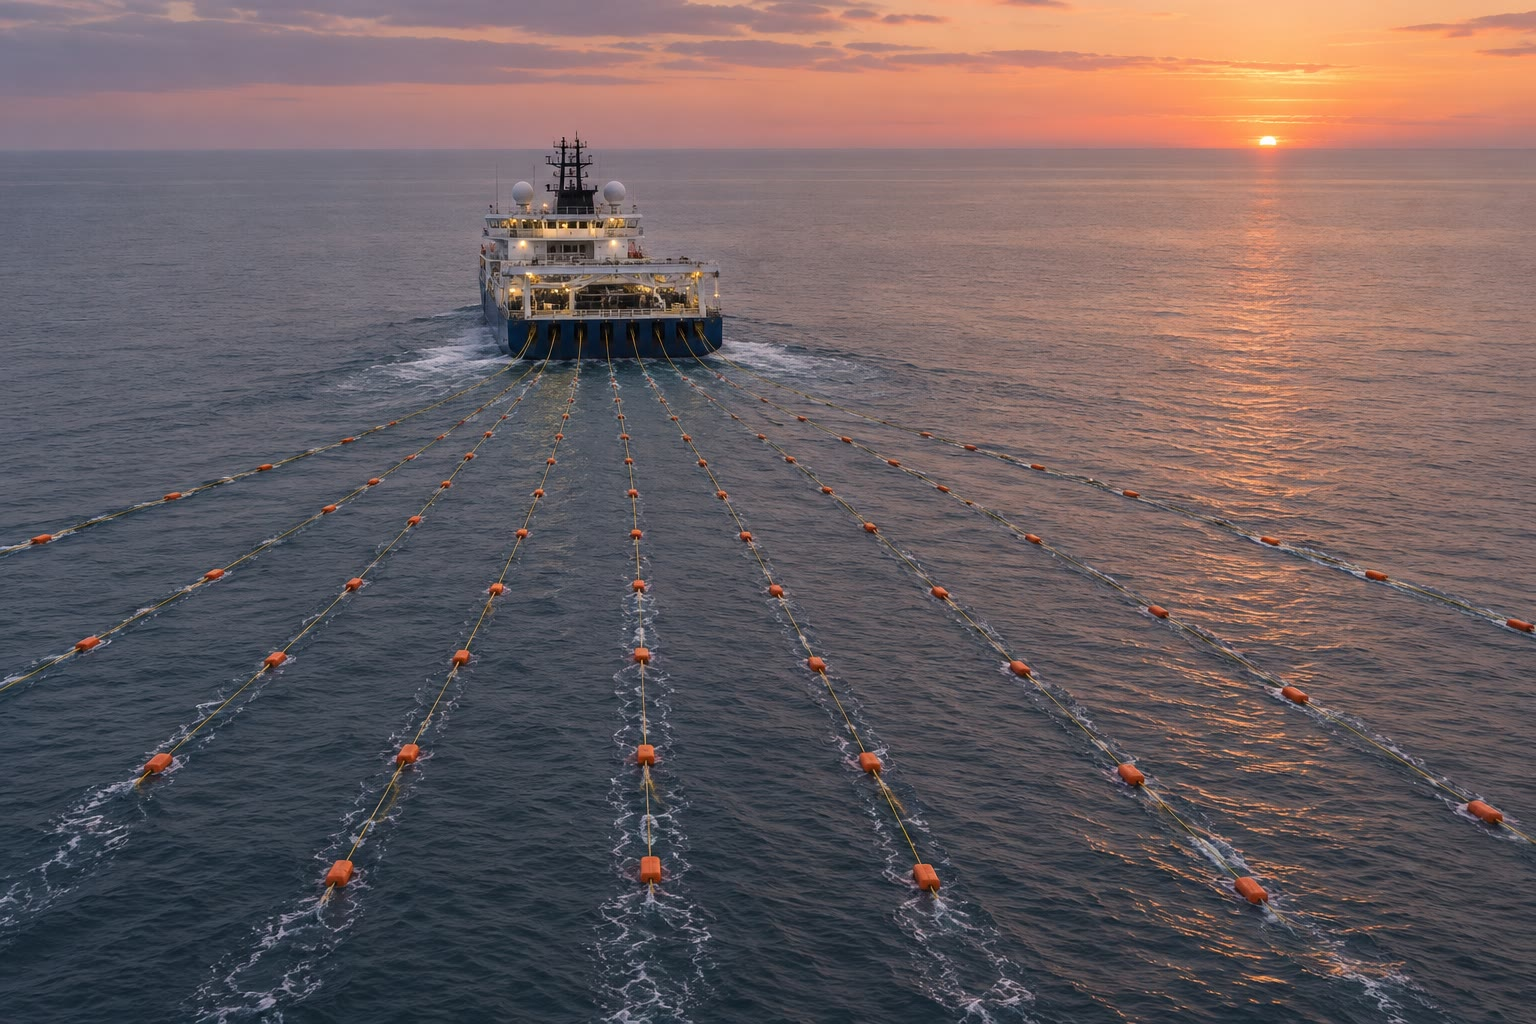
\includegraphics[width=\linewidth]{images/book5/ai/b3-streamer-vessel.jpg}

{\scriptsize भूकंपीय सर्वेक्षण का एक जहाज़ गोधूलि में अपने स्ट्रीमर खींचता हुआ
(AI से बनाया गया चित्रण)।}
\end{minipage}
\end{inthefield}

\section{अभ्यास}

\begin{exercise}[$\star$]\label{exo:b3:exploration-seismology:1}
चॉक ($v = \qty{2500}{m.s^{-1}}$, $\rho = \qty{2.00}{g.cm^{-3}}$) शेल पर स्थित है,
(\qty{2300}{m.s^{-1}}, \qty{2.30}{g.cm^{-3}}), जो चूना-पत्थर पर स्थित है
(\qty{4500}{m.s^{-1}}, \qty{2.60}{g.cm^{-3}})। तीनों प्रतिबाधाएँ और
दोनों अंतरापृष्ठों के परावर्तन गुणांक ज्ञात कीजिए। आपतित ऊर्जा का कितना भाग
चूना-पत्थर की ऊपरी सतह परावर्तित करती है?
% ledger: mavko:velocities
\end{exercise}

\begin{exercise}[$\star$]\label{exo:b3:exploration-seismology:2}
एक समतल परावर्तक \qty{800}{m} गहराई पर स्थित है, जो \qty{2000}{m.s^{-1}} वेग की परत के नीचे है।
\qty{1000}{m} विस्थापन पर परावर्तन काल $t_0$, और वहाँ का \omterm{thm:b3:exploration-seismology:nmo}{सामान्य
मूवआउट} ज्ञात कीजिए, और सन्निकटन $x^2/(2v^2t_0)$ से तुलना कीजिए।
\end{exercise}

\begin{exercise}[$\star$]\label{exo:b3:exploration-seismology:3}
एक स्ट्रीमर में 240 चैनल हैं, जिनकी दूरी \qty{12.5}{m} है, और जहाज़ हर
\qty{25}{m} पर स्रोत दागता है। CMP अंतराल और आच्छादन गुणक ज्ञात कीजिए।
कौन-सा शॉट अंतराल 120 का आच्छादन गुणक देगा?
\end{exercise}

\begin{exercise}[$\star$]\label{exo:b3:exploration-seismology:4}
\qty{30}{Hz} की प्रमुख आवृत्ति पर तरंगदैर्घ्य और
\qty{3000}{m.s^{-1}} वेग वाले बलुआ पत्थर में चतुर्थांश तरंगदैर्घ्य और
\qty{4500}{m.s^{-1}} वेग वाले चूना-पत्थर में चतुर्थांश तरंगदैर्घ्य ज्ञात कीजिए। \qty{1000}{m} गहरे
परावर्तक के लिए, \qty{2800}{m.s^{-1}} माध्य वेग वाली चट्टानों के नीचे, प्रथम \omterm{def:b3:exploration-seismology:fresnel}{फ़्रेनेल क्षेत्र} की त्रिज्या ज्ञात कीजिए।
\end{exercise}

\begin{exercise}[$\star\star$]\label{exo:b3:exploration-seismology:5}
दो परावर्तनों में से एक का $t_0 = \qty{0.500}{s}$ है, और उसका \omterm{def:b3:exploration-seismology:velocities}{वर्ग-माध्य-मूल वेग}
\qty{2400}{m.s^{-1}} है; दूसरे का $t_0 = \qty{0.700}{s}$ है, और उसका \omterm{def:b3:exploration-seismology:velocities}{वर्ग-माध्य-मूल वेग} \qty{2800}{m.s^{-1}} है।
\omterm{def:b3:exploration-seismology:velocities}{अंतराल वेग} और इन दोनों के बीच की परत की मोटाई ज्ञात कीजिए।
\end{exercise}

\begin{exercise}[$\star\star$]\label{exo:b3:exploration-seismology:6}
CMP रेखा के तल में एक समतल परावर्तक $\varphi$ कोण पर नत है, जो
वेग $v$ वाली परत में है। (क) दिखाइए कि $t(x)^2 = t_0^2 + x^2\cos^2\varphi/v^2$ है, जहाँ $t_0$
मध्यबिंदु पर शून्य-विस्थापन काल है। (संकेत: परावर्तक में मध्यबिंदु के
प्रतिबिंब का उपयोग कीजिए।) (ख) \omterm{def:b3:exploration-seismology:velocities}{स्टैकिंग वेग} निकालिए, और उसे
$v = \qty{2000}{m.s^{-1}}$ और $\varphi = \ang{12}$ के लिए ज्ञात कीजिए।
\end{exercise}

\begin{exercise}[$\star\star$]\label{exo:b3:exploration-seismology:7}
आच्छादन गुणक 60 वाले एक संग्रह के हर अनुरेख पर समान प्रसरण का स्वतंत्र शोर है। स्टैकिंग से
सिग्नल-से-शोर अनुपात किस गुणक से बढ़ता है? उसे फिर दोगुना करने के लिए आच्छादन गुणक किस गुणक से
बढ़ाना होगा?
\end{exercise}

\begin{exercise}[$\star\star$]\label{exo:b3:exploration-seismology:8}
शून्य-विस्थापन काल खंड पर, \qty{3000}{m.s^{-1}} वेग वाली चट्टान में, एक परावर्तन
रेखा के अनुदिश प्रति किलोमीटर \qty{0.40}{s} द्वि-मार्ग काल की दर से ऊपर उठता है। इस ढलान को
आभासी नति में बदलिए, और परावर्तक की वास्तविक नति ज्ञात कीजिए।
\end{exercise}

\begin{exercise}[$\star\star$]\label{exo:b3:exploration-seismology:9}
\omterm{def:b3:exploration-seismology:synthetic}{परावर्तकता श्रेणी} $r = (0, 0.3, 0, -0.2, 0)$ को
तीन-नमूना वाली तरंगिका $w = (-0.5, 1, -0.5)$ के साथ नमूने-दर-नमूने संवलित कीजिए। दोनों
परावर्तन कहाँ हैं, और क्या वे अतिव्यापित होते हैं?
\end{exercise}

\begin{exercise}[$\star\star\star$]\label{exo:b3:exploration-seismology:10}
\qty{1800}{m.s^{-1}} वेग की परत के ऊपर एक उलटा अपवर्तन परिच्छेद
नति की दिशा में आभासी वेग \qty{2900}{m.s^{-1}} और नति के विपरीत आभासी वेग
\qty{4400}{m.s^{-1}} देता है। क्रांतिक कोण, नति और परावर्तक का
वेग ज्ञात कीजिए। परावर्तक के वेग की
दोनों आभासी वेगों के हरात्मक माध्य से तुलना कीजिए।
\end{exercise}

\begin{exercise}[$\star\star\star$]\label{exo:b3:exploration-seismology:11}
\cref{prop:b3:exploration-seismology:tuning} में एक संस्तर के परावर्तन गुणांक
$+R$ और $-R$ हैं। (क) दिखाइए कि $\Delta t \ll T$ के लिए मिश्रित संकेत
लगभग $R\,\Delta t\,w'(t)$ है, जो तरंगिका का समय-अवकलज है,
जिसे संस्तर की द्वि-मार्ग मोटाई से गुणा किया गया है। (ख) समझाइए कि पतला संस्तर
विभेदित न होने पर भी पहचाना जा सकता है, और उसके आयाम से उसकी मोटाई का अनुमान कैसे लगाया जा सकता है।
(ग) एक ही चट्टान के, 5 और \qty{10}{m} मोटाई वाले दो संस्तर एक ही तरंगिका से
प्रतिबिंबित किए गए हैं: उनके आयामों का अनुपात क्या है?
\end{exercise}

\begin{exercise}[$\star\star\star$]\label{exo:b3:exploration-seismology:12}
एक बिंदु प्रकीर्णक रेखा के \qty{600}{m} नीचे, वेग
\qty{3000}{m.s^{-1}} वाली चट्टान में स्थित है। (क) उसके विवर्तन का शून्य-विस्थापन काल, बिंदु के ठीक ऊपर से क्षैतिज दूरी $x$ के
विरुद्ध लिखिए, और उसे $x = 0$ तथा
\qty{300}{m} पर ज्ञात कीजिए। (ख) दिखाइए कि विवर्तन NMO रूप का एक अतिपरवलय है
जिसका वेग $v/2$ है, और समझाइए कि विवर्तन सदा समान शीर्ष-काल वाले किसी
परावर्तन से अधिक वक्र क्यों होता है। (ग) \omterm{def:b3:exploration-seismology:migration}{भूकंपीय माइग्रेशन} इस पर क्या करता है?
\end{exercise}

\section{समस्या: वार्डन पहाड़ियों के आर-पार एक भूकंपीय रेखा}

\begin{problem}[{सप्ताहांत समस्या --- अपवर्तन, वेग विश्लेषण, गहराई रूपांतरण और माइग्रेशन,
वार्डन पहाड़ियों के खंड A--B के अनुदिश}]
\label{pb:b3:exploration-seismology:1}
% values: calc/ch02.py, from figdata seismic_model.py, refraction_dip.py, cmp_nmo.py
यह भूकंपीय रेखा वार्डन पहाड़ियों के खंड A--B के अनुदिश चलाई गई है, वह क्षेत्र जिसके
भूवैज्ञानिक मानचित्र पिछले खंडों में दिए गए हैं। इसकी दूरियाँ $s$ रेखा के अनुदिश
A से गिनी जाती हैं। ऊपर से आवरण चॉक, शेल (\qty{100}{m}),
चूना-पत्थर (\qty{180}{m}) और बलुआ पत्थर (\qty{120}{m}) हैं, जो असंगति के साथ
एक शिस्ट आधारशैल पर टिके हैं; यह अपनति और अभिनति में मुड़ी है, और
एक सामान्य भ्रंश से कटी है।

\medskip
\noindent\textbf{भाग I --- पश्चिमी भुजा पर एक अपवर्तन विस्तार।} एक
\qty{1200}{m} का विस्तार शॉट बिंदुओं W ($s = \qty{300}{m}$) और E
($s = \qty{1500}{m}$) के बीच बिछाया गया है, और भूमि को समतल माना गया है। चूना-पत्थर के ऊपर
के चॉक और शेल को एक परत माना गया है, जिसका $v_1 = \qty{2.40}{km.s^{-1}}$ वेग है। अभिलेखों पर
पढ़े गए हेड तरंग काल, W से E की ओर, \qty{800}{m} पर \qty{425.2}{ms} और
\qty{1200}{m} पर \qty{486.1}{ms}; E से W की ओर,
\qty{800}{m} पर \qty{372.4}{ms} और \qty{1200}{m} पर \qty{486.1}{ms} हैं।
\begin{enumerate}
  \item दोनों आभासी वेग ज्ञात कीजिए। कौन-सा शॉट ऊपर-नति की दिशा में है?
  \item परावर्तक का क्रांतिक कोण और नति ज्ञात कीजिए।
  \item परावर्तक का वेग ज्ञात कीजिए। यह कौन-सी चट्टान है?
  \item W और E के नीचे परावर्तक के अंतःखंड काल और लंबवत गहराइयाँ
        ज्ञात कीजिए।
  \item इन्हें ऊर्ध्वाधर गहराइयों में बदलिए, और दोनों गहराइयों से नति की जाँच कीजिए।
  \item चॉक के नीचे का शेल चॉक से धीमा है। \omterm{def:b3:exploration-seismology:surveys}{भूकंपीय अपवर्तन सर्वेक्षण} इसे क्या
        समझता है, और यह गहराइयों में कैसा पूर्वाग्रह उत्पन्न करता है?
\end{enumerate}

\noindent\textbf{भाग II --- CMP S पर वेग विश्लेषण।} और आगे पूर्व की ओर, CMP S
अभिनति के अक्ष पर, भ्रंश के अवनत खंड में स्थित है,
जहाँ स्तरों को समतल माना गया है। चार परावर्तन शून्य-विस्थापन और
\qty{600}{m} पर चुने गए हैं:
\begin{center}
\small
\begin{tabular}{lcccc}
\hline
परावर्तन & 1 & 2 & 3 & 4 \\
$t_0$ (\unit{s}) & 0.4878 & 0.5748 & 0.6548 & 0.7348 \\
$t(\qty{600}{m})$ (\unit{s}) & 0.5437 & 0.6240 & 0.6887 & 0.7648 \\
\hline
\end{tabular}
\end{center}
\begin{enumerate}[resume]
  \item परावर्तन 1 और 2 के NMO वेग $V = x/\sqrt{t^2 - t_0^2}$ परिकलित कीजिए।
        दूसरा मान पहले से छोटा क्यों है?
  \item परावर्तन 3 और 4 के लिए इसे परिकलित कीजिए।
  \item इन्हें \omterm{def:b3:exploration-seismology:velocities}{वर्ग-माध्य-मूल वेग} मानकर प्रत्येक परत का \omterm{def:b3:exploration-seismology:velocities}{अंतराल वेग}
        \omterm{thm:b3:exploration-seismology:dix}{डिक्स समीकरण} से परिकलित कीजिए।
  \item उनके वेगों से परतों की पहचान कीजिए, और चारों परावर्तक
        अंतरापृष्ठों के नाम बताइए।
  \item परावर्तन 1 अभिलेखों पर सबसे क्षीण है। क्यों?
  \item वेग केवल \qty{600}{m} तक के विस्थापनों पर ही क्यों मापे गए,
        जबकि प्रसार \qty{2}{km} तक पहुँचता है?
\end{enumerate}

\noindent\textbf{भाग III --- गहराई में रूपांतरण और विभेदन।}
\begin{enumerate}[resume]
  \item प्रत्येक परत में लगा द्वि-मार्ग काल और उसकी मोटाई परिकलित कीजिए।
  \item भूतल के नीचे प्रत्येक परावर्तक अंतरापृष्ठ की गहराई परिकलित कीजिए।
        शेल, चूना-पत्थर और बलुआ पत्थर की मोटाइयों की तुलना ऊपर दिए
        मानों से कीजिए।
  \item भूतल से आधारशैल तक का माध्य वेग परिकलित कीजिए, और समझाइए कि यदि
        इसके स्थान पर परावर्तन 4 का NMO वेग प्रयोग किया जाए, तो गहराई का
        अधिक आकलन क्यों होगा।
  \item सर्वेक्षण की तरंगिका का शिखर \qty{30}{Hz} पर है। शेल में तरंगदैर्घ्य
        और उसकी \omterm{def:b3:exploration-seismology:resolution}{समस्वरण मोटाई} चौथाई-तरंगदैर्घ्य नियम से और \omterm{def:b3:exploration-seismology:wavelet}{रिकर तरंगिका} के
        लिए $b = v/(5.2f)$ द्वारा, दोनों प्रकार से परिकलित कीजिए। क्या शेल
        विभेदित है? किस आवृत्ति पर यह चौथाई-तरंगदैर्घ्य नियम से समस्वरित होगा?
  \item परावर्तन 4 के NMO वेग से $\lambda$ लेकर, आधारशैल पर प्रथम \omterm{def:b3:exploration-seismology:fresnel}{फ़्रेनेल
        क्षेत्र} की त्रिज्या परिकलित कीजिए।
\end{enumerate}

\noindent\textbf{भाग IV --- भूकंपीय माइग्रेशन और भ्रंश।}
\begin{enumerate}[resume]
  \item भ्रंश के निकट चूना-पत्थर की कटाव-सीमा से एक विवर्तन उत्पन्न होता है,
        जिसका शीर्ष \qty{0.550}{s} पर है; शीर्ष से रेखा के अनुदिश \qty{200}{m} दूर
        वह \qty{0.5732}{s} पर है। शून्य-विस्थापन विवर्तन काल लिखिए और
        कटाव-सीमा के ऊपर का माध्य वेग निकालिए।
  \item भूतल के नीचे कटाव-सीमा की गहराई परिकलित कीजिए।
  \item पूर्वी पक्ष पर स्टैक्ड खंड का ऊपरी चूना-पत्थर परावर्तन अपनति की ओर
        प्रति किलोमीटर \qty{0.167}{s} द्वि-मार्ग काल से ऊपर उठता है,
        जो माध्य वेग \qty{2.48}{km.s^{-1}} वाली चट्टानों में है। इसका आभासी नति और
        वास्तविक नति परिकलित कीजिए।
  \item उस पक्ष पर एक परावर्तन $t = \qty{0.655}{s}$ पर अभिलिखित है। माइग्रेशन
        उसे कितना और किस दिशा में विस्थापित करता है?
  \item भ्रंश के आर-पार ऊपरी आधारशैल परावर्तन \qty{0.160}{s} की छलाँग लगाता है;
        अवनत खंड में चॉक की अतिरिक्त मोटाई है। भ्रंश का विस्थापन
        परिकलित कीजिए।
  \item भाग II के अंतराल वेगों से CMP S के नीचे आधारशैल असंगति की
        गहराई दीजिए।
\end{enumerate}
\end{problem}
